\subsection{How individual examples were selected}
We chose the shirt, helmeted dog and jar in main Fig.~3 after inspecting the outputs. Their requests change a color, add flowers to the dog's mouth and open a lid, respectively. Figure~\ref{fig:v19-ranked-changes} separately retains the original example-selection rule. It ranks all 50 sources on two contrasts in directional CLIP (uniform minus constants and spatial minus constants) and selects cases near high, middle and low joint ranks. The painting has a full edit mask. Its background score is undefined, whereas its embedding response and whole-image change are measurable.

\begin{figure*}[t]\centering
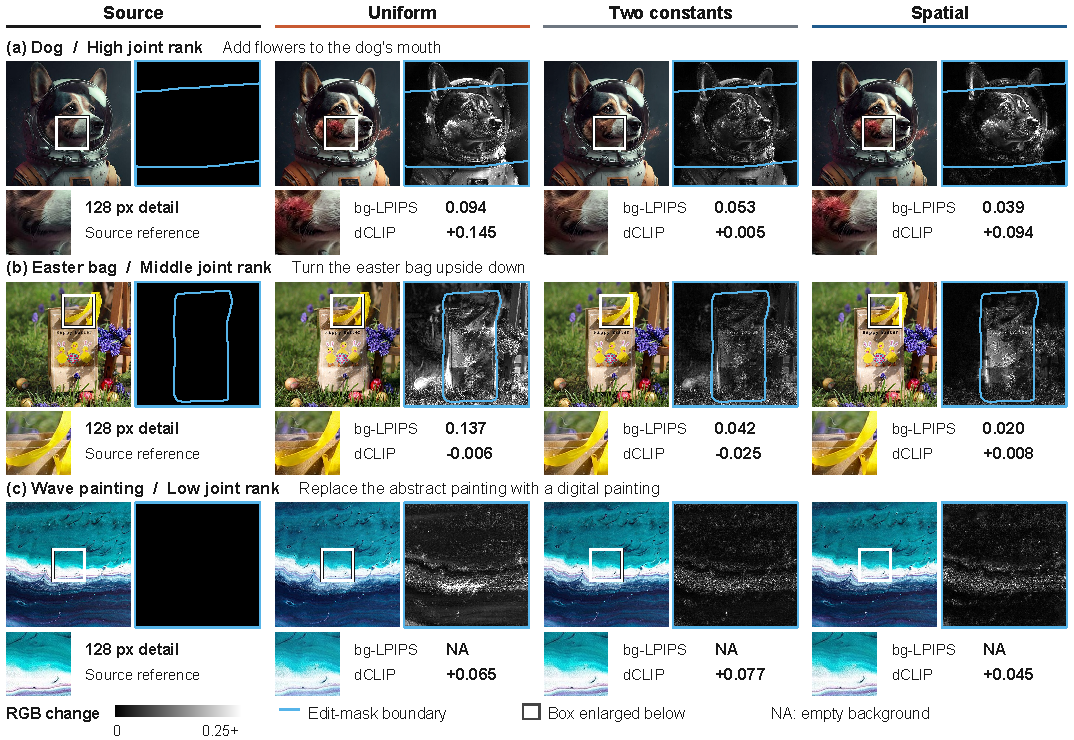
\includegraphics[width=\textwidth]{figures/v19_changes_ranked.pdf}
\caption{A high joint-rank dog, a middle-rank bag and a low-rank painting under the original selection rule. The bag stays upright under all three configurations. Scores beside the crops are regional feature-map LPIPS and directional CLIP. All maps share the same absolute RGB scale across images and configurations.}
\label{fig:v19-ranked-changes}
\end{figure*}
\begin{figure*}[t]\centering
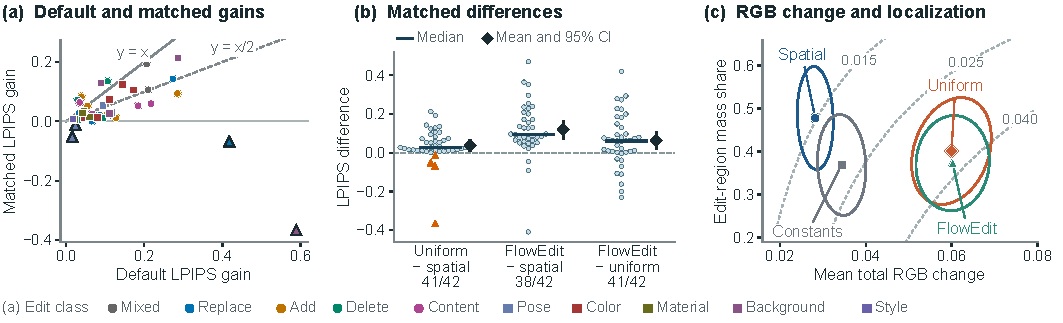
\includegraphics[width=\textwidth]{figures/v19_response.pdf}
\caption{The size of the response-matching adjustment varies by source. Panel (a) pairs default and matched gaps within each image. Panel (b) shows all three configuration contrasts. The last panel shows total pixel change and its concentration on the 42 nonempty backgrounds. The common spatial LPIPS field supplies the background measure throughout.}
\label{fig:v19-response-sensitivity}
\end{figure*}
